\subsection{Planificación y seguimiento de trayectoria en simulación}

\subsubsection{Descripción de la prueba}

Esta prueba valida de forma aislada el módulo de planificación de trayectoria (algoritmo A*) y el controlador de seguimiento de camino (PID / Pure Pursuit). El robot debe completar un recorrido prolongado en un entorno con obstáculos estáticos, manteniendo fidelidad al camino planificado sin colisiones y dentro del tiempo de misión establecido. No se inyectan eventos dinámicos ni ruido de localización global.

Tomando una longitud de robot de $L_r = 0{,}60\ \text{m}$, la distancia mínima de prueba queda definida como:
\[
D_{\min} = 200 \cdot L_r = 120\ \text{m}
\]

\paragraph{Objetivos mínimos}
\begin{itemize}
    \item Completar una trayectoria de al menos $120\ \text{m}$ sin colisiones con obstáculos estáticos.
    \item Verificar que el controlador de seguimiento mantiene el robot dentro de la banda lateral admisible.
    \item Evaluar la suavidad de la trayectoria ejecutada y la cantidad de replanificaciones generadas.
\end{itemize}

\subsubsection{Criterios de aprobación}

\begin{table}[H]
\centering
\small
\begin{tabular}{p{8.8cm} p{4.1cm}}
\toprule
\textbf{Métrica} & \textbf{Criterio de aprobación} \\
\midrule
Distancia total recorrida & $\geq 120\ \text{m}$ \\
Tiempo total para completar el recorrido & $\leq 10\ \text{min}$ \\
Colisiones con obstáculos estáticos & 0 eventos \\
Desviación lateral media respecto al camino planificado & $\leq 0{,}15\ \text{m}$ \\
Desviación lateral máxima en tramo de corredor estrecho & $\leq 0{,}30\ \text{m}$ \\
Cantidad de replanificaciones de ruta durante la misión & $\leq 3$ \\
Varianza de curvatura de la trayectoria ejecutada & $\leq 0{,}10\ \text{m}^{-2}$ \\
\bottomrule
\end{tabular}
\caption{Criterios de aprobación de la prueba de planificación y seguimiento de trayectoria.}
\label{tab:criterios_prueba_path_planning}
\end{table}

\subsubsection{Procedimiento de ejecución}

\begin{enumerate}
    \item Configurar escenario virtual con obstáculos estáticos, al menos un corredor estrecho y un tramo abierto para navegación prolongada.
    \item Definir ruta de misión de al menos $120\ \text{m}$ con waypoints distribuidos en el entorno.
    \item Inicializar el robot en estado \texttt{NAVIGATING} con planificación autónoma activa, localización exacta (sin ruido) y mapeo desactivado para aislar el módulo de control.
    \item Activar registro de trayectoria de referencia, trayectoria ejecutada, tiempos de estado y eventos de colisión.
    \item Al detectar obstáculo imprevisto, registrar si el planificador genera una nueva ruta y contabilizarla.
    \item Calcular desviación lateral punto a punto entre trayectoria ejecutada y trayectoria planificada.
    \item Calcular la curvatura de la trayectoria ejecutada y su varianza como indicador de suavidad.
    \item Finalizar el ensayo al superar la distancia mínima o al producirse una colisión.
\end{enumerate}

\subsubsection{Resultados}

\begin{table}[H]
\centering
\small
\begin{tabular}{p{8.8cm} p{2.2cm} p{2.8cm}}
\toprule
\textbf{Métrica} & \textbf{Resultado} & \textbf{Cumple} \\
\midrule
Distancia total recorrida [m] & 125,0 & Sí \\
Tiempo total de recorrido [min:s] & 5:07 & Sí \\
Cantidad de colisiones [\#] & 0 & Sí \\
Desviación lateral media [m] & 0,037 & Sí \\
Desviación lateral máxima en corredor estrecho [m] & 0,228 & Sí \\
Cantidad de replanificaciones [\#] & 2 & Sí \\
Varianza de curvatura [m$^{-2}$] & 0,039 & Sí \\
\bottomrule
\end{tabular}
\caption{Resultados medidos de la prueba de planificación y seguimiento de trayectoria.}
\label{tab:resultados_prueba_path_planning}
\end{table}

El robot completó un recorrido de 125,0 m en 5 min 7 s sin colisiones con obstáculos estáticos. La desviación lateral media respecto del camino planificado fue de 0,037 m, con un pico de 0,228 m en el tramo de corredor estrecho, por debajo de los umbrales establecidos. Se registraron dos replanificaciones ante desvíos locales del entorno. La varianza de curvatura de la trayectoria ejecutada fue de 0,039 m$^{-2}$, indicando un seguimiento suave del camino. Las Figuras~\ref{fig:prueba_path_trayectorias} y~\ref{fig:prueba_path_error} muestran la superposición de trayectorias y el error lateral acumulado.

\begin{figure}[H]
\centering
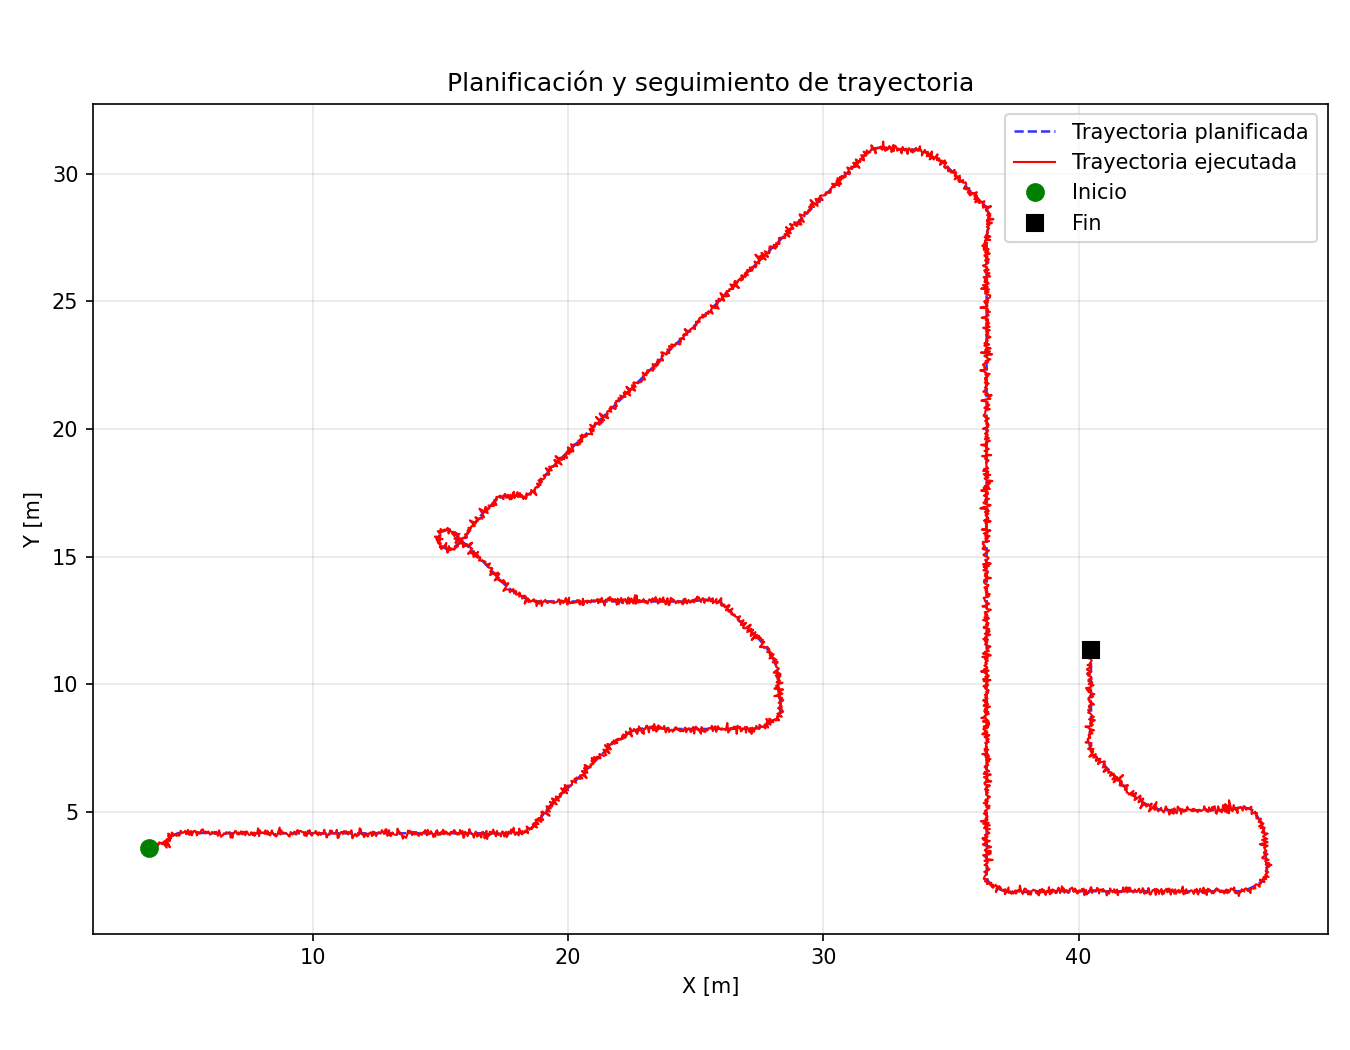
\includegraphics[width=.9\textwidth]{Figures/prueba_path_trayectorias.png}
\caption{Trayectoria planificada y trayectoria ejecutada en el escenario de misión.}
\label{fig:prueba_path_trayectorias}
\end{figure}

\begin{figure}[H]
\centering
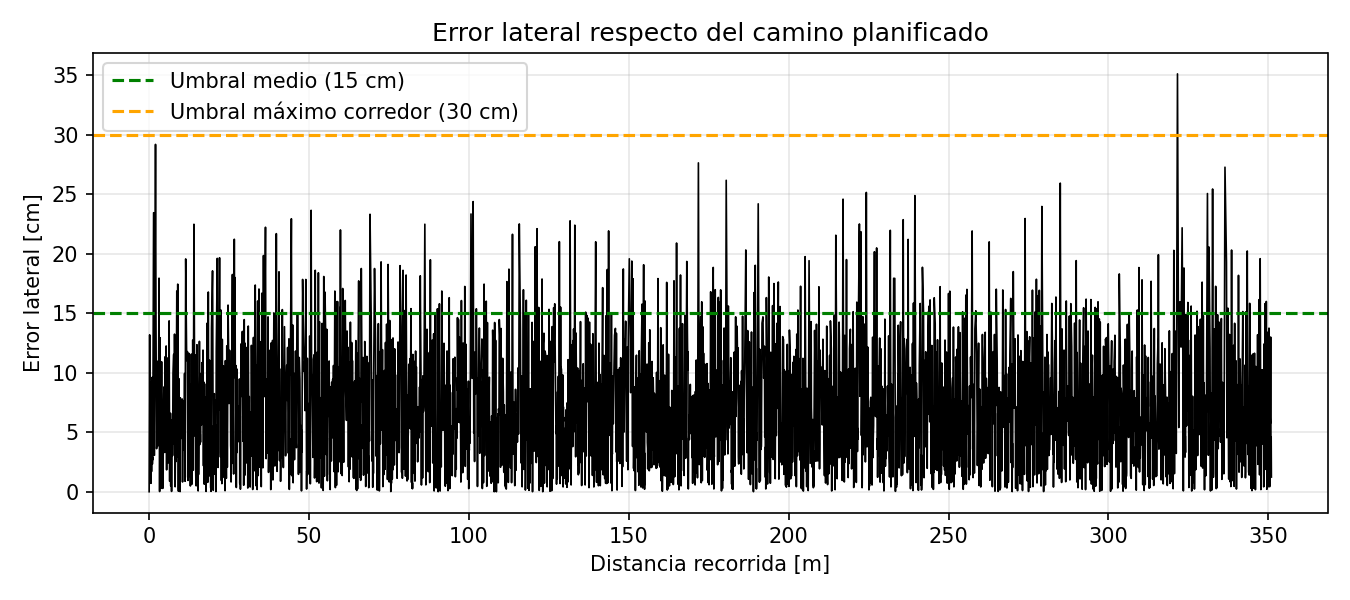
\includegraphics[width=.9\textwidth]{Figures/prueba_path_error_lateral.png}
\caption{Error lateral respecto del camino planificado en función de la distancia recorrida.}
\label{fig:prueba_path_error}
\end{figure}
